\usetikzlibrary{arrows.meta,positioning,matrix}

\newcommand{\nodepair}[2]{\textbf{#1}\\\footnotesize #2}

\tikzset{
base node/.style={
draw=black!68,
thick,
rounded corners=2.5pt,
align=center,
font=\footnotesize,
inner sep=3pt,
minimum height=8.5mm,
text width=2.15cm
},
module/.style={base node, fill=blue!12},
data/.style={base node, fill=green!12, text width=2.05cm},
component/.style={base node, fill=yellow!18, text width=2.25cm},
flowarrow/.style={-{Latex[length=2.1mm,width=1.7mm]}, semithick, draw=black!72},
rewardarrow/.style={-{Latex[length=2.5mm,width=2.0mm]}, very thick, draw=black!90},
controlarrow/.style={-{Latex[length=2.0mm,width=1.6mm]}, thin, draw=blue!60!black!75},
edgelabel/.style={font=\footnotesize, fill=white, inner sep=1pt, rounded corners=1pt}
}

\begin{figure*}[!tbp]
\centering
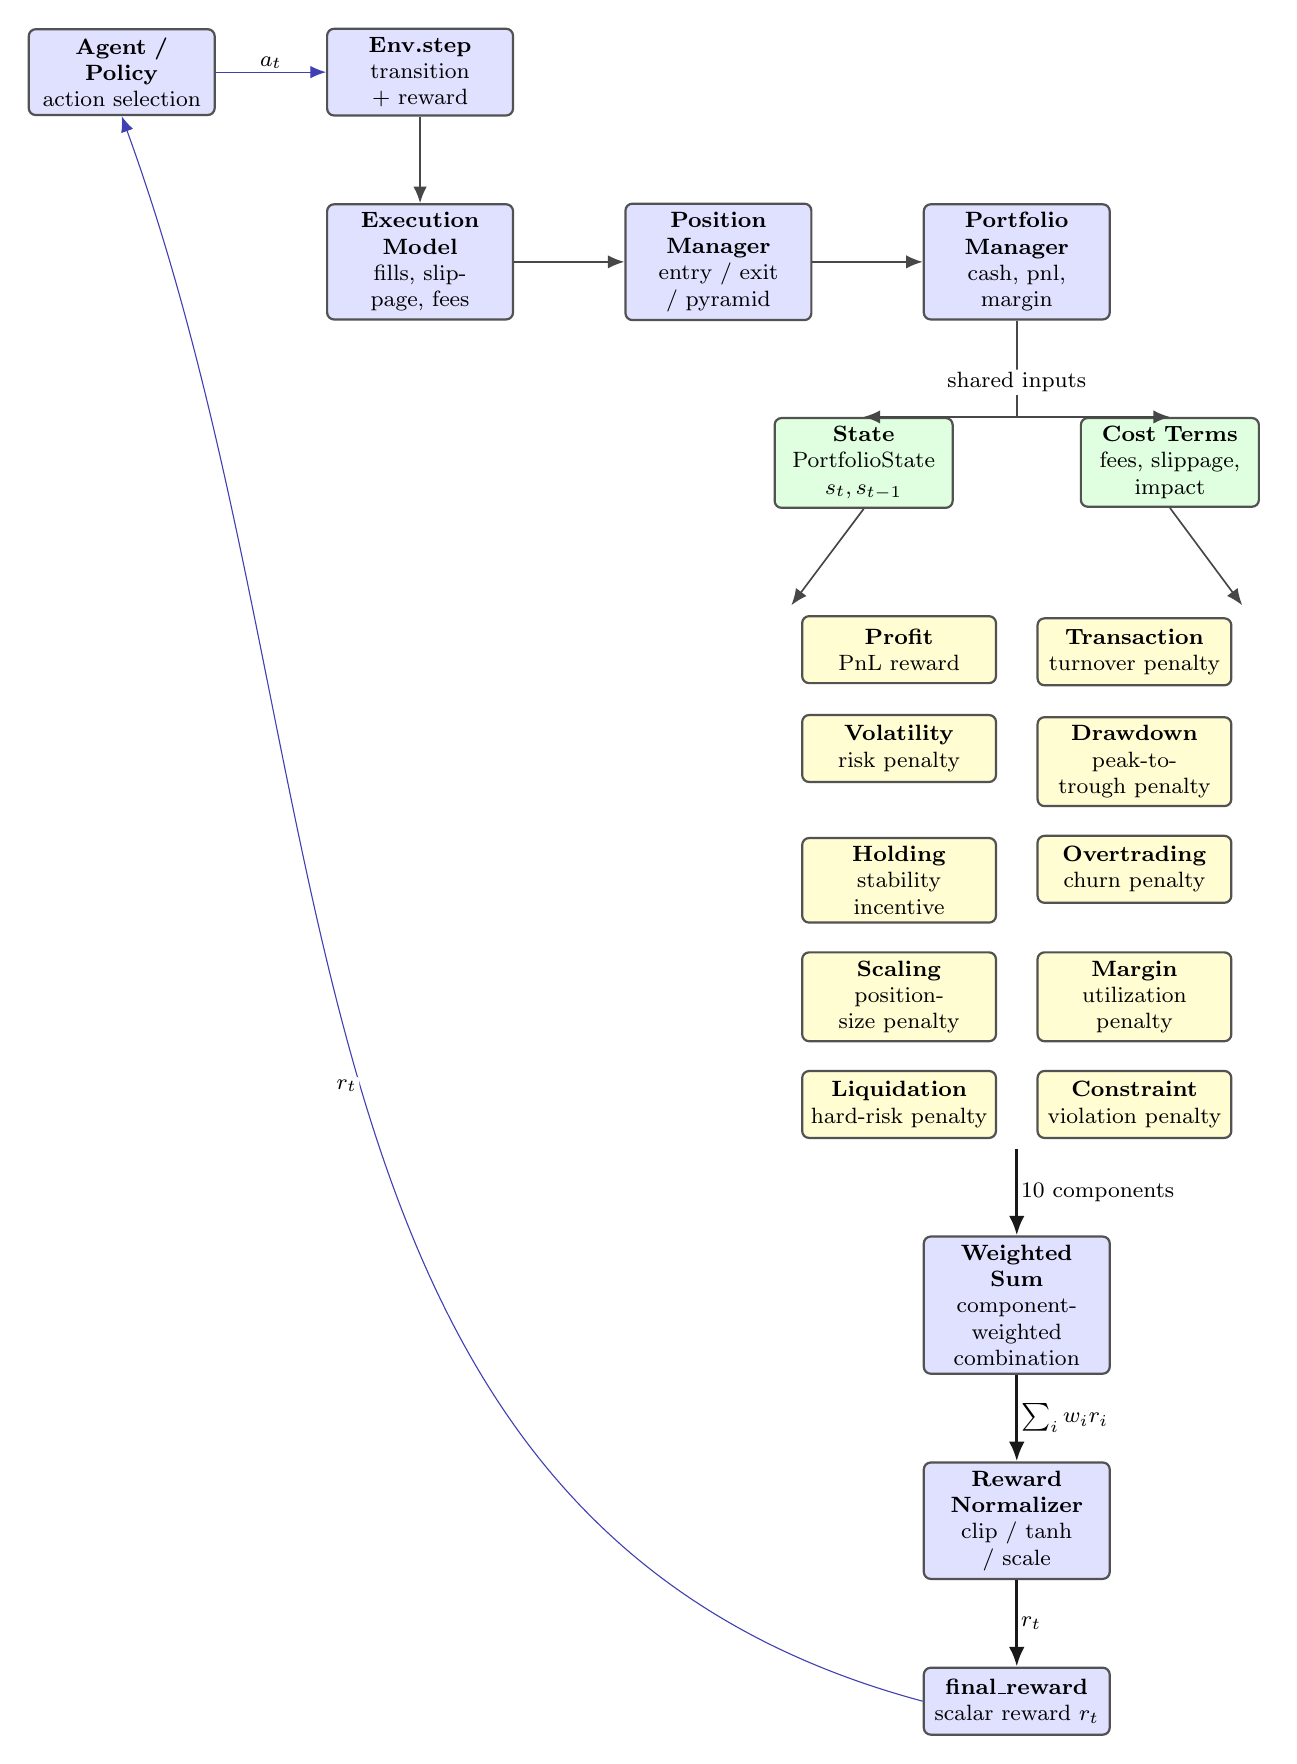
\begin{tikzpicture}[node distance=11mm and 14mm]

% ========== ROW 1: AGENT INTERACTION ==========
\node[module] (agent) {\nodepair{Agent / Policy}{action selection}};
\node[module, right=of agent] (envstep) {\nodepair{Env.step}{transition + reward}};

% ========== ROW 2: EXECUTION & PORTFOLIO ==========
\node[module, below=of envstep] (exec) {\nodepair{Execution Model}{fills, slippage, fees}};
\node[module, right=of exec] (pos) {\nodepair{Position Manager}{entry / exit / pyramid}};
\node[module, right=of pos] (portfolio) {\nodepair{Portfolio Manager}{cash, pnl, margin}};

\matrix (sharedinputs) [matrix of nodes,
nodes={data},
column sep=16mm,
below=of portfolio,
anchor=north] {
|[alias=state]|{\nodepair{State}{PortfolioState $s_t, s_{t-1}$}} &
|[alias=cost]|{\nodepair{Cost Terms}{fees, slippage, impact}} \\
};

% ========== ROW 3: REWARD COMPONENTS GRID (CENTRAL FOCAL BLOCK) ==========
\matrix (rewardgrid) [matrix of nodes,
nodes={component},
column sep=5mm,
row sep=3.5mm,
below=of sharedinputs,
anchor=north] {
|[alias=pnl]|         {\nodepair{Profit}{PnL reward}} &
|[alias=transaction]| {\nodepair{Transaction}{turnover penalty}} \\
|[alias=vol]|         {\nodepair{Volatility}{risk penalty}} &
|[alias=drawdown]|    {\nodepair{Drawdown}{peak-to-trough penalty}} \\
|[alias=holding]|     {\nodepair{Holding}{stability incentive}} &
|[alias=overtrade]|   {\nodepair{Overtrading}{churn penalty}} \\
|[alias=scaling]|     {\nodepair{Scaling}{position-size penalty}} &
|[alias=margin]|      {\nodepair{Margin}{utilization penalty}} \\
|[alias=liq]|         {\nodepair{Liquidation}{hard-risk penalty}} &
|[alias=constraint]|  {\nodepair{Constraint}{violation penalty}} \\
};

% ========== ROW 4: REWARD AGGREGATION ==========
\node[module, below=of rewardgrid] (sum) {\nodepair{Weighted Sum}{component-weighted combination}};
\node[module, below=of sum] (norm) {\nodepair{Reward Normalizer}{clip / tanh / scale}};
\node[module, below=of norm] (final) {\nodepair{final\_reward}{scalar reward $r_t$}};

% ========== PRIMARY TOP-TO-BOTTOM FLOW ==========
\draw[controlarrow] (agent) -- node[edgelabel, above] {$a_t$} (envstep);
\draw[flowarrow] (envstep) -- (exec);
\draw[flowarrow] (exec) -- (pos);
\draw[flowarrow] (pos) -- (portfolio);
\draw[flowarrow] (portfolio.south) |- (state.north);
\draw[flowarrow] (portfolio.south) |- (cost.north);

\draw[flowarrow] (state.south) -- (rewardgrid.north west);
\draw[flowarrow] (cost.south) -- (rewardgrid.north east);
\node[edgelabel, above=1.5mm of sharedinputs.north] {shared inputs};

% Dominant reward computation path
\draw[rewardarrow] (rewardgrid.south) -- node[edgelabel, right] {10 components} (sum.north);
\draw[rewardarrow] (sum) -- node[edgelabel, right] {$\sum_i w_i r_i$} (norm);
\draw[rewardarrow] (norm) -- node[edgelabel, right] {$r_t$} (final);

% Secondary feedback (de-emphasized)
\draw[controlarrow] (final.west) to[out=165,in=-70] node[edgelabel, left] {$r_t$} (agent.south);

\end{tikzpicture}

\caption{Reward taxonomy and computation flow for the RL trading environment, from agent--environment interaction through component aggregation and normalization to the final scalar reward.}\label{fig:reward_taxonomy}
\end{figure*}